\begin{figure}[t]
\centering
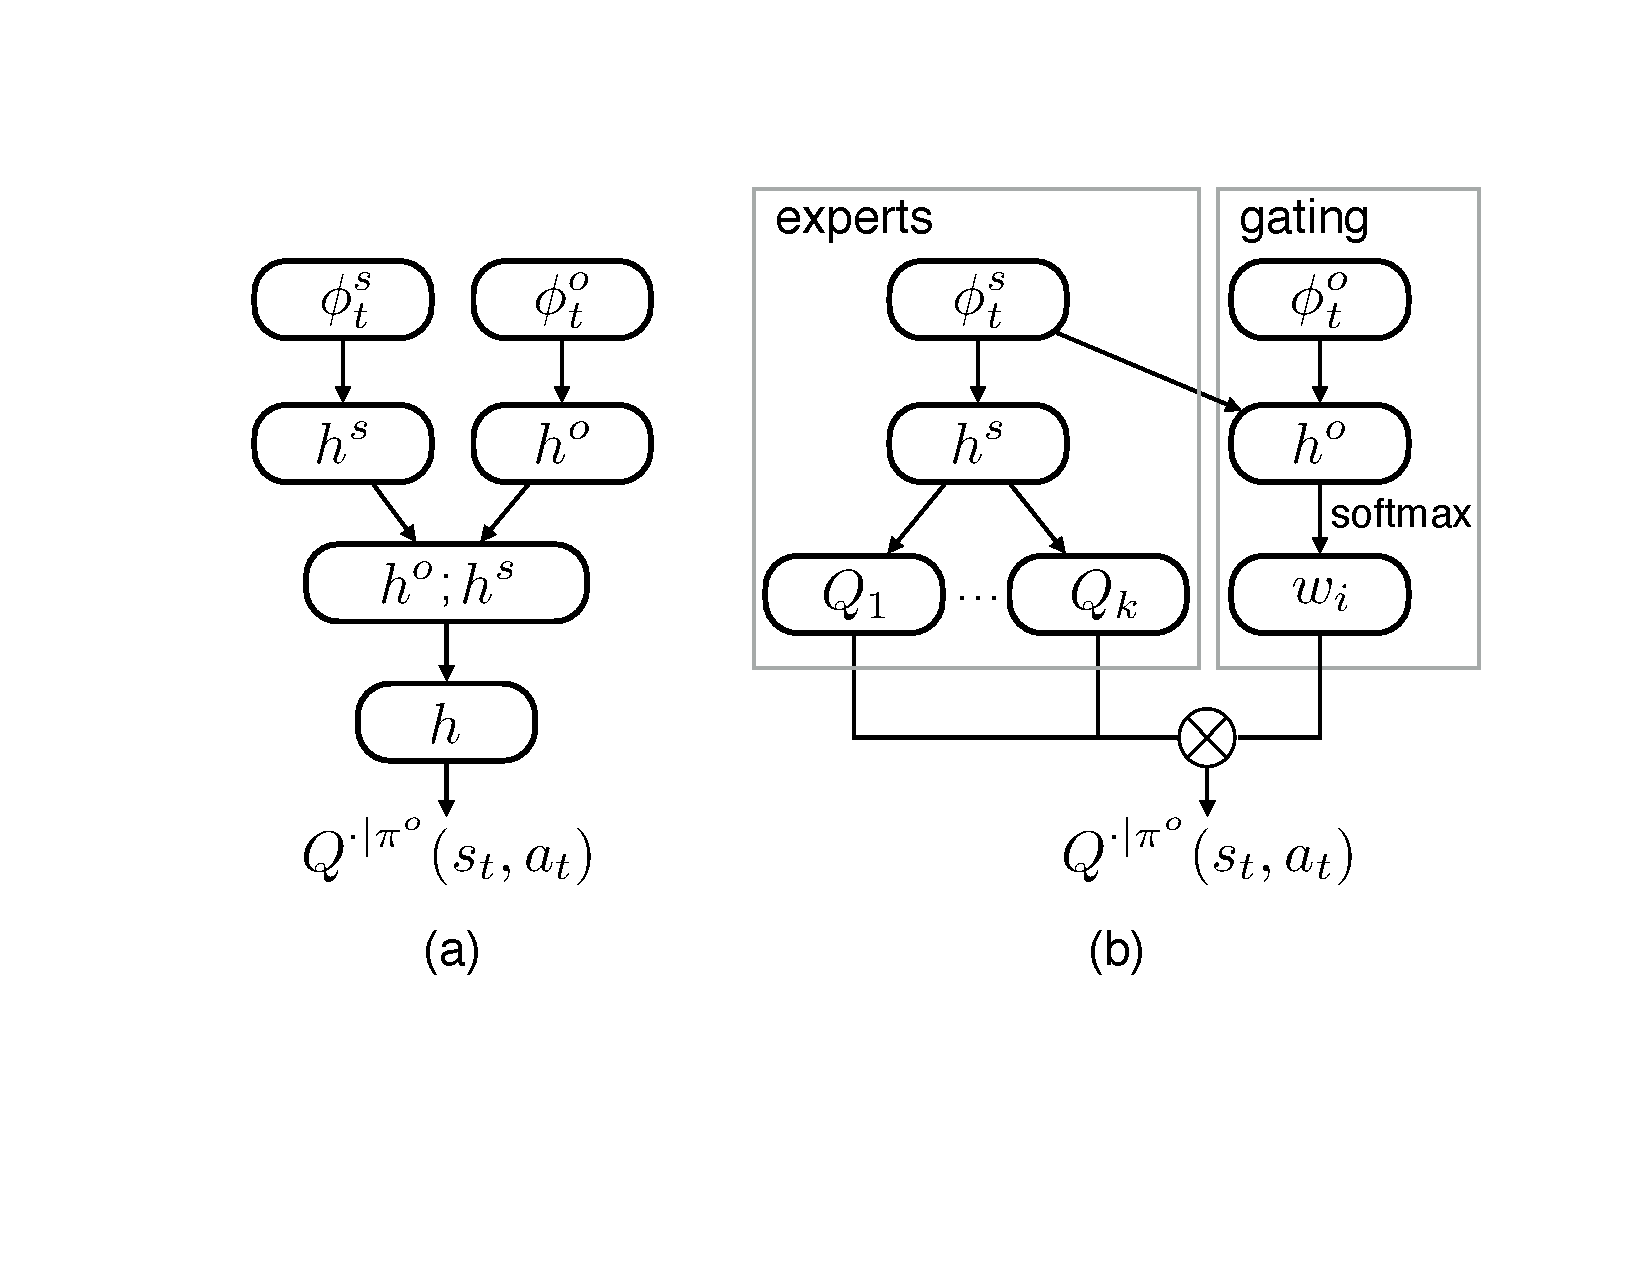
\includegraphics[width=0.42\textwidth]{2016_icml_opponent/figures/opp_networks}
\caption{Diagram of the \dron{} architecture. (a) \dron{}-concat: opponent representation is concatenated with the state representation.
(b) \dron{}-MoE: Q-values predicted by $K$ experts are combined linearly by weights from the gating network.}
\label{fig:dron}
\end{figure}

\begin{figure}[t]
\centering
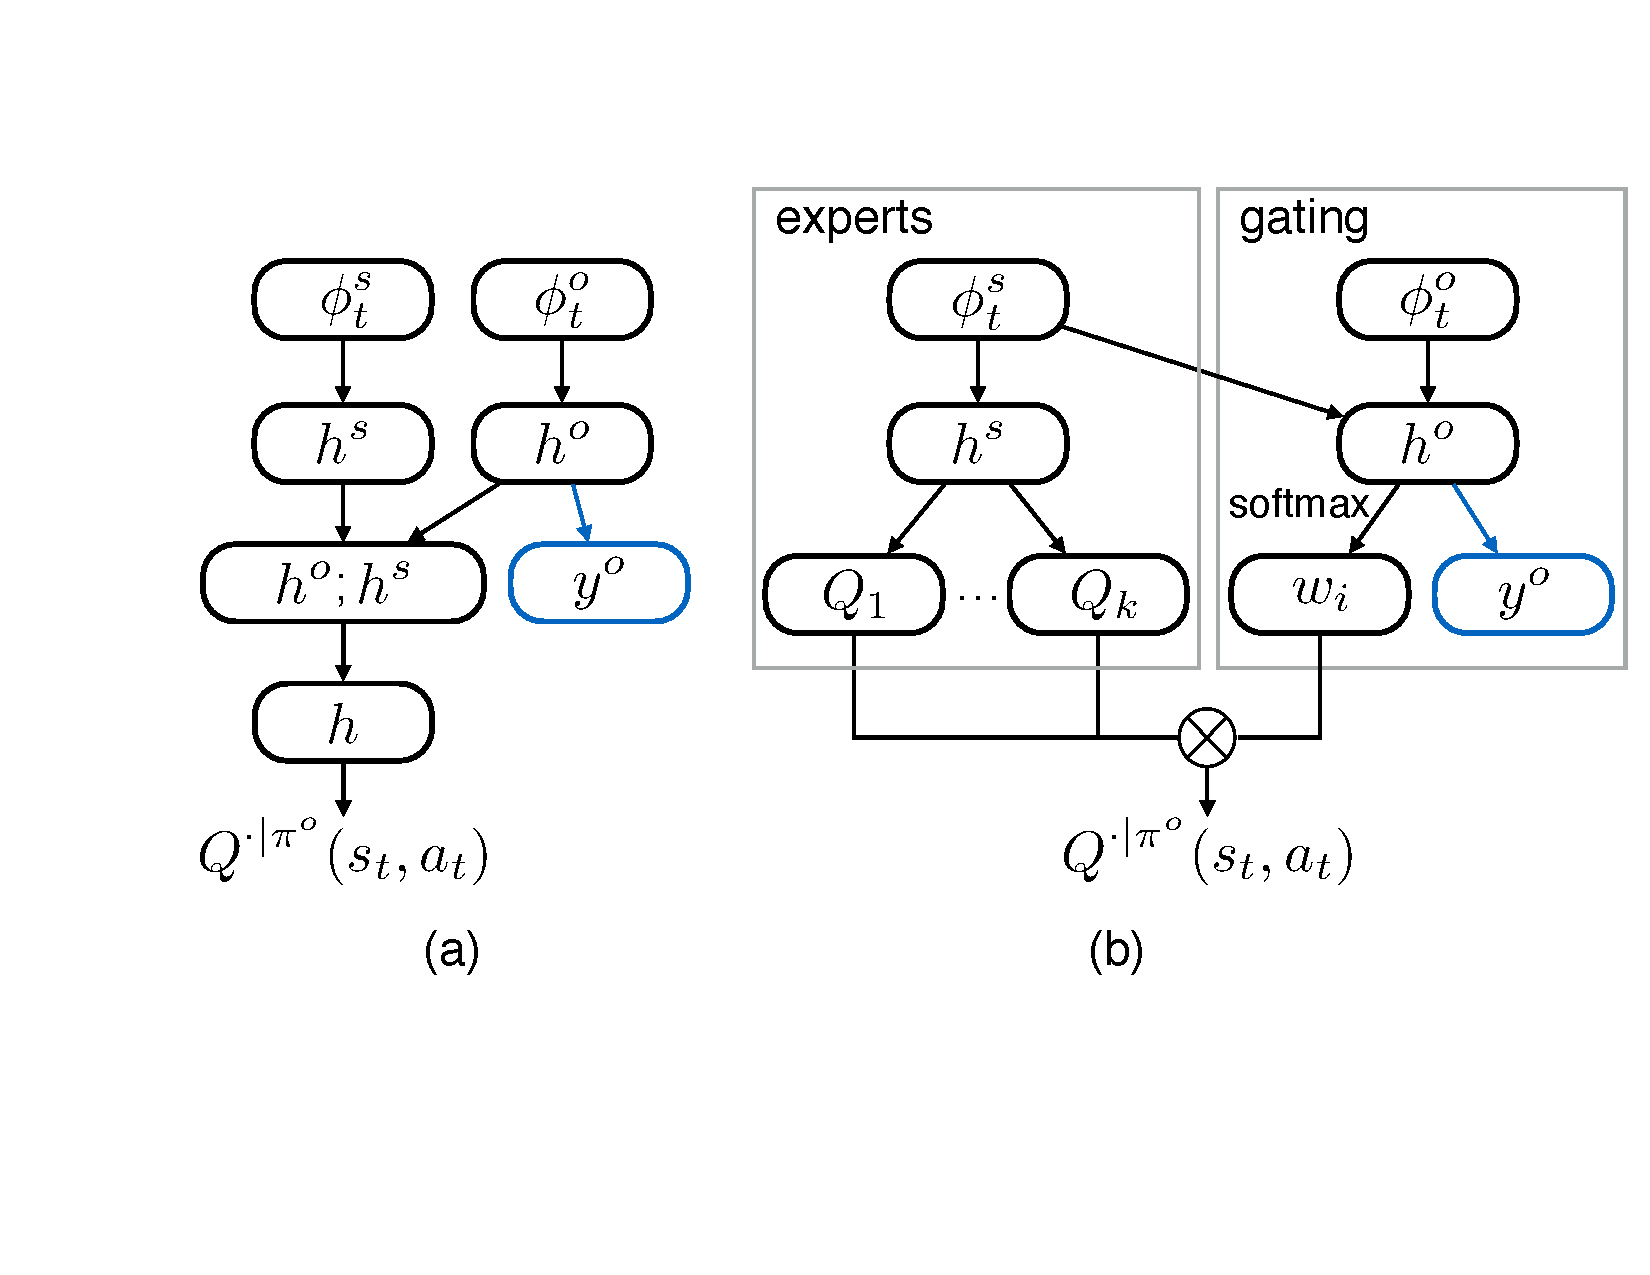
\includegraphics[width=0.48\textwidth]{2016_icml_opponent/figures/opp_networks_mt}
\caption{Diagram of the DRON with multitasking. The blue part shows that the supervision signal from the opponent affects the Q-learning network by changing the opponent features.}
\label{fig:dron-mt}
\end{figure}


\section{Deep Reinforcement Opponent Network}
\label{sec:method}

In a multi-agent setting, the environment is affected by the \emph{joint} action
of all agents.  From the perspective of one agent, the outcome of an action in a
given state is no longer stable, but is dependent on actions of other agents.
In this section, we first analyze the effect of multiple agents on the Q-learning framework;
then we present \dron{} and its multitasking variation.

\subsection{Q-Learning with Opponents}

In \abr{mdp} terms, the joint action space is defined by $\mathcal{A}^M =
\mathcal{A}_1 \times \mathcal{A}_2 \times \ldots \times \mathcal{A}_n$ where $n$
is the total number of agents.  We use $a$ to denote the action of the agent we
control (the primary agent) and $\oa$ to denote the joint action of all other agents (secondary agents), such that $(a,
\oa) \in \mathcal{A}^M$.  Similarly, the transition probability becomes
$\mathcal{T}^M(s,a,\oa,s')=Pr(s'|s,a,\oa)$, and the new reward function is
$\mathcal{R}^M(s,a,\oa,s')$.  Our goal is to learn an optimal policy for the primary
agent given interactions with the joint policy $\op$ of the secondary
agents.\footnote{While a joint policy defines the distribution of joint actions,
  the opponents may be controlled by independent policies.}

If $\op$ is stationary, then the multi-agent \abr{mdp} reduces to a single-agent
\abr{mdp}: the opponents can be considered part of the world.  Thus, they
redefine the transitions and reward:
\begin{eqnarray*}
\mathcal{T}(s,a,s')&=&\sum_{\oa} \op(\oa|s) \mathcal{T}^M(s,a,\oa,s'), \\
\mathcal{R}(s,a,s')&=&\sum_{\oa} \op(\oa|s) \mathcal{R}^M(s,a,\oa,s').
\end{eqnarray*}
Therefore, an agent can ignore other agents,
and standard Q-learning suffices.

Nevertheless, it is often unrealistic to assume opponents use fixed
policies.  Other agents may also be learning or adapting to maximize rewards.
For example, in strategy games, players may disguise their true
strategies at the beginning to fool the opponents; winning players
protect their lead by playing defensively; and losing players play
more aggressively.  In these situations, we face opponents with an unknown
policy $\op_t$ that changes over time.

Considering the effects of other agents, the definition of an optimal policy in
Section~\ref{sec:background} no longer applies---the effectiveness policies now
depends on policies of secondary agents.  We therefore define the optimal
$Q$-function relative to the joint policy of opponents: $Q^{\ast|\op} =
\max_{\pi} Q^{\pi|\op}(s,a) \; \forall s \in \mathcal{S} \;\mbox{and}\; \forall
a \in \mathcal{A}$.  The recurrent relation between Q-values holds:
\begin{eqnarray}
Q^{\pi|\op}(s_t,a_t) = \sum_{\oa_t} \op_t(\oa_t|s_t) \sum_{s_{t+1}} \mathcal{T}(s_t,a_t,\oa_t,s_{t+1}) \nonumber \\
\left[ \mathcal{R}(s_t,a_t,\oa_t,s_{t+1}) + \gamma\e{a_{t+1}}{Q^{\pi|\op}(s_{t+1},a_{t+1})} \right] .
\label{eqn:opponent-q}
\end{eqnarray}

\subsection{DQN with Opponent Modeling}

Given Equation~\ref{eqn:opponent-q}, we can continue applying Q-learning and
estimate both the transition function and the opponents' policy by stochastic
updates.  However, treating opponents as part of the world can slow
responses to adaptive opponents~\cite{opponent-qlearning}, because
the change in behavior is masked by the dynamics of the world.

To encode opponent behavior explicitly, we propose the Deep
Reinforcement Opponent Network (\dron{}) that models $Q^{\cdot|\op}$
and $\op$ jointly.  \dron{} is a Q-Network ($N_Q$) that
evaluates actions for a state and an opponent network ($N_o$) that
learns representation of $\op$.  The remaining questions are how to
combine the two networks and what supervision signal to use.  To
answer the first question, we investigate two network architectures:
\dron{}-concat that concatenates $N_Q$ and $N_o$, and \dronmoe{} that
applies a Mixture-of-Experts model.



To answer the second question, we consider two settings:
(a) predicting Q-values only, as our goal is the best reward instead of accurately simulating opponents;
and (b) also predicting extra information about the opponent when it is available, e.g., the type of their strategy.

\paragraph{\dron-concat}

We extract features from the state ($\phi^s$) and the opponent ($\phi^o$ ) and
then use linear layers with rectification or convolutional neural networks---$N_Q$ and $N_o$---to embed them
in separate hidden spaces ($h^s$ and $h^o$).
To incorporate knowledge of $\op$ into the Q-Network,
we concatenate representations of the
state and the opponent (Figure~\ref{fig:dron}a).  The
concatenation then jointly predicts the Q-value.  Therefore, the last layer(s) of the neural
network is responsible for understanding the interaction between opponents and
Q-values.  Since there is only one Q-Network, the model requires a more discriminative representation of the opponents to learn an adaptive policy.
To alleviate this, our second model encodes a
stronger prior of the relation between opponents' actions and Q-values based on Equation~\ref{eqn:opponent-q}.

\paragraph{\dronmoe}

The right part of Equation~\ref{eqn:opponent-q} can be written as
$\sum_{\oa_t} \op_t(\oa_t|s_t) Q^\pi(s_t,a_t,\oa_t)$, an expectation
over different opponent behavior.  We use a
Mixture-of-Experts network~\cite{moe} to explicitly model the opponent
action as a hidden variable and marginalize over it
(Figure~\ref{fig:dron}b).  The expected Q-value is obtained by
combining predictions from multiple \emph{expert networks}:
\begin{eqnarray*}
Q(s_t, a_t; \theta) &=& \sum_{i=1}^K w_i Q_i(h^s, a_t) \\
Q_i(h^s, \cdot) &=& f(W_i^s h^s + b_i^s) .
\end{eqnarray*}
Each expert network predicts a possible reward in the current state.
A \emph{gating network} based on the opponent representation computes combination weights (distribution over experts):
\begin{equation*}
w = \mbox{softmax}\left(f(W^o h^o + b^o)\right).
\end{equation*}
Here $f(\cdot)$ is a nonlinear activation function (ReLU for
all experiments),
$W$ represents the linear transformation matrix, and $b$ is the bias term.

Unlike \dron{}-concat, which ignores the interaction between the world and
opponent behavior, \dronmoe{} knows that Q-values have different distributions
depending on $\phi^o$; each expert network captures one type of
opponent strategy.

\paragraph{Multitasking with \dron{}}





The previous two models
predict Q-values only, thus the opponent representation is learned
indirectly through feedback from the Q-value.  Extra information
about the opponent can provide direct supervision for $N_o$.
Many games reveal additional information besides the
final reward at the end of a game.  At the very least the agent has
observed actions taken by the opponents in past states; sometimes
their private information such as the hidden cards in poker.  More high-level
information includes abstracted plans or strategies.
Such information reflects characteristics of opponents and
can aid policy learning.

Unlike previous work that learns a separate model to predict these
information about the
opponent~\cite{davidson99opponent,game-theory-opponent-modeling,schadd07opponentmodeling},
we apply multitask learning and use the observation as extra
supervision to learn a \emph{shared} opponent representation
$h^o$.  Figure~\ref{fig:dron-mt} shows the architecture of multitask
\dron{}, where supervision is $y^o$.
The advantage of multitasking over explicit opponent modeling is that
it uses high-level knowledge of the game and the opponent, while
remaining robust to insufficient opponent data and modeling error
from Q-values.  In Section~\ref{sec:experiments},
we evaluate multitasking \dron{} with two types of supervision
signals: future action and overall strategy of the opponent.
